\documentclass{article}

\usepackage{summary}

\subject{Urheberrecht in der Informationsgesellschaft}
\semester{Summer 2024}
\author{Leopold Lemmermann}

\begin{document}\createtitle



\section{Geistiges Eigentum}
\begin{quote}
  Zeitlich beschränkter Schutz immateriellen, geistigen Inhalts. In Abgrenzung zu Sachenrechten, die sich auf materielle Gegenstände beziehen und zeitlich unbeschränkt sind.
\end{quote}

\begin{itemize}
  \item Ideelles Persönlichkeitsrecht: nicht veräußerlich \& zeitlich begrenzt
  \item Materielle, wirtschaftliche Rechte: Ansprüche.
\end{itemize}

Territorialität: Keine einheitliche Rechtsordnung, sondern nationale Gesetze.

Rechtsgrundsätze: lex-specialis, lex-posterior, lex-superior

\subsection{Normenpyramide im Urheberrecht}

Internationale Verträge: Universal Copyright Convention, TRIPS, WIPO Copyright Treaty, Berner Übereinkunft\\
Europarecht: diverse Richtlinien\\
Nationale Gesetze: UrhG, VGG, VerlG

\subsection{Kritik an EU-Reform von 2019}
Artikel 15 (Leistungsschutzrecht): Lizenzierungspflicht für Texte führt evtl. zu weniger Medienvielfalt.\\
Artikel 17 (Uploadfilter): Plattformbetreiber müssen Inhalte präventiv filtern, was zu Overblocking führen kann.

\subsection{Urheberrechts-Dienstanbieter-Gesetz (UrhDaG)}
Kritik an EU-Reform verarbeiten.
Lösungansatz
\begin{itemize}
  \item Blockierung nicht-lizenzierter Uploads: grds. erlaubte Nutzung annehmen (gg. Overblocking), per Red Button sofortiges Blockieren durch Rechteinhaber
  \item Meinungs- \& Kommunikationsfreiheit durhc präzisierte Schranken.
\end{itemize}
Ausnahmen für geringfügige Nutzung oder Satire, Parodie, etc…

\begin{figure}
  \resizebox{\textwidth}{!}{
    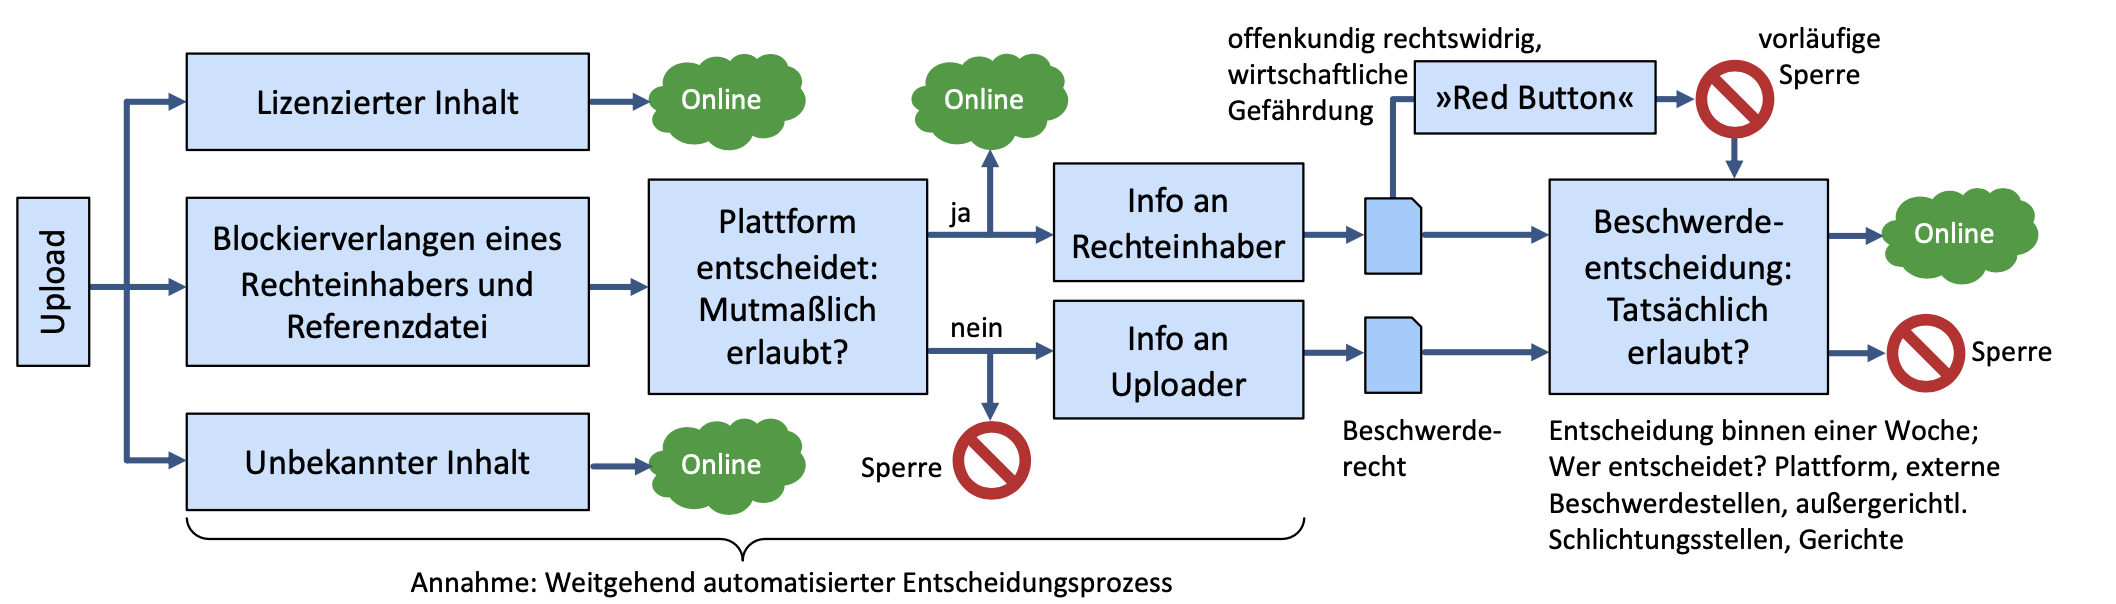
\includegraphics{res/uploads.png}
  }
  \caption{Uploads}
\end{figure}



\section{Urheberrechtsgesetz (UrhG)}
\begin{table}
  \centering
  \begin{tabular}{c|c|c|c|c}
    §§1-69       & §§70-87h           & §§88-95 & §§96-119              & §§120-143            \\
    Urheberrecht & verw. Schutzrechte & Filme   & geteilte Bestimmungen & Anwendungsbereich, …
  \end{tabular}
\end{table}

Kaum formelle Anforderungen, Copyrightvermerk nicht notwendig (aber verbreitet für Rechtsdurchsetzung). Gewerbliche Schutzrechte sind (zumeist) anmeldepflichtig.

\subsection{Werkbegriff (§2 II UrhG)}
Urheberrecht i.e.S. umfasst Werke, d.h. persönlich-geistige Schöpfungen, die individuellen Charakter haben:
\begin{itemize}
  \item Literatur, Wissenschaft, Kunst
  \item Menschlich-gestalterische Leistung: nicht allein durch Maschine erstellt
  \item Geistiger Gehalt
  \item Form: konkret \& wahrnehmbar
  \item Individualität: Unterscheidbarkeit von anderen Werken
\end{itemize}

\subsection{Besondere Werke}
\begin{itemize}
  \item Computerprogramme (Art. 1 III RL 2009/24/EG): Individuelles Werk aus geistiger Schöpfung des Urhebers genügt
  \item Datenbanken (Art. 3 I RL 96/9/EG): Feststellbare geistige Schöpfung in Auswahl oder Anordnung genügt
  \item Lichtbilder (§72 UrhG): Schutz als Lichtbildwerk, wenn individuelle Schöpfung
\end{itemize}

\section{Computerprogramme (§69a-g UrhG)}

\begin{itemize}
  \item[a)] I. Programme verstanden einschließlich Entwurfsmaterial etc.
        II. Gilt für alle Ausdrucksformen. Aber keine allgemeinen Ideen, sondern nur konkrete Ausdrucksformen.
        III. geistige Schöpfung ausschlaggebend, insb. nicht Ästhetik oder Qualität.
  \item[b)] grds. Arbeitgeber als Urheber
  \item[c)] Zustimmungsbedürftige Handlungen: Verfielfältigung, Übersetzung etc., Verbreitung, Öffentlichmachen
  \item[d)] Ausnahmen: bestimmte Nutzung/Fehlerberichtigung, berechtigte Sicherheitskopie, Programmtestläufe
  \item[e)] Dekompilierung für Interoperatibilität: Schnittstellen finden
  \item[f)] Rechtsverletzung: Vernichtungsanspruch, Schutz vor Umgehung von Kopierschutz
  \item[g)] sonstiges Recht weiterhin angewendet
\end{itemize}



\section{Recht am eigenen Bild}
\subsection{Sphärentheorie \& Schutzwürdigkeit}
\begin{enumerate}
  \item Intimsphäre (stärkster)
  \item Privatsphäre (stark): häuslicher Bereich, Familienkreis, Privatleben
  \item Sozialsphäre (schwach): Mensch als soziales Wesen
  \item Öffentlichkeitssphäre (schwächster): bewusst öffentlich
\end{enumerate}

\subsection{Recht am eigenen Bild (KunstUrhG)}
\begin{itemize}
  \item[§22 1] Bilder nur mit Einwilligung verarbeiten
  \item[§22 3] von Geburt bis 10 Jahre nach dem Tod
  \item[§23 I] Ausnahmen: Öffentliche Veranstaltungen, Zeitgeschichte, Kunst
  \item[§23 II] Aber trotzdem berechtigtes Interesse zu berücksichtigen
\end{itemize}



\section{Lizenzierung}

\subsection{Urhebervertrag (nach UrhG)}
\begin{itemize}
  \item[§29] grds. unübertragbar, aber diverse Nutzungsrechte
  \item[§31 II] einfaches Nutzungsrecht: teilen mit anderen möglich
  \item[§31 III] ausschließliches Nutzungsrecht: nur der Lizenznehmer
\end{itemize}

\subsubsection{Urhebervertrag in der Praxis}
\begin{itemize}
  \item Vertragszweck \& Werk
  \item Rechtseinräumungsumfang: einfach/ausschließlich, zeitlich/räumlich/inhaltlich, Dritte, unbekannte Nutzungsarten
  \item Arten: Verfielfältigung, Veröffentlichung, Bearbeitung
  \item Vergütung: pauschal/Beteiligung, Höhe, Abrechnungszyklus
  \item Gewährleistung, Haftung/-freistellung
  \item Rechtswahl, Gerichsstand
\end{itemize}

\subsubsection{Abstraktions- vs. Kausalitätsprinzip}
\begin{itemize}
  \item Abstraktionsprinzip (Vertrag \& Rechtseinräumung getrennt): Gilt allgemein, im UrhR umstritten
  \item Kausalitätsprinzip (Vertrag \& Rechtseinräumung gemeinsam)
\end{itemize}

Gutgläubiger Erwerb im UrhR ausgeschlossen $\to$ lückenlose Vertragskette

\subsection{Freie Lizenzen}
Copyleft: gleiche Lizenz für abgeleitete Werke

\begin{itemize}
  \item \textbf{CC} (Creative Commons): standardisierte nicht-reversible Nutzungserlaubnis (Rechtsgrundlage §32 III 3 UrhG)
  \item \textbf{GPL} (GNU General Public License): Copyleft für Software
  \item \textbf{DL-DE}: Datennutzungslizensen für offene Daten
\end{itemize}

\begin{itemize}
  \item \textbf{CC}: BY (Attribution), SA (Share-Alike), NC (Non-Commercial), ND (No Derivates)
  \item \textbf{DL-DE}: BY (Attribution) \& 0 (Public)
\end{itemize}

\subsection{Nutzung von Internetmaterial}
\subsubsection{Wo?}
\begin{itemize}
  \item beim Urheber = Rechteinhaber
  \item bei Dritten (sukzessiver Rechteinhaber, Verwertungsgesellschaften)
  \item Registrierung bei EUIPO
  \item Innerhalb von Organisation durch internen Prozess
\end{itemize}

\subsubsection{Wie?}
\begin{enumerate}
  \item Rechteinhaber identifizieren
  \item Anfrage mit Nutzungszweck
  \item Verhandlung über Nutzungsbedingungen, insb. Gebühr
  \item Lizenzvertrag
  \item Vertragsschluss \& Erfüllung
  \item bei zeitlicher Beschränkung: Verlängerung
\end{enumerate}



\section{Schranken}

\subsection{Prinzipien}
\begin{enumerate}
  \item bestimmte Einzelfälle
  \item normale Auswertung unbeeinträchtigt
  \item berechtigte Interessen des Urhebers nicht beeinträchtigt
\end{enumerate}

\subsection{Arten}
\begin{itemize}
  \item \textbf{GL} (Gesetzliche Lizenz): Nutzung einwilligungsfrei, aber mit Vergütung
  \item \textbf{FS} (Freistellung): Nutzung erlaubnis- \& vergütungsfrei
\end{itemize}

\subsection{Schranken des UrhG}
\begin{itemize}
  \item[§44a] (FS) Vorübergehende Vervielfältigungshandlungen: Browser-Cache, Text-/Data Mining
  \item[§45] (FS) Rechtspflege und öffentliche Sicherheit: keine Behinderung öffentlicher Aufgaben
  \item[§45a] (GL) Behinderte Menschen: barrierefreie Nutzung
  \item[§46] (GL)  Sammlungen für den religiösen Gebrauch: Vergütungspflicht, Mitteilung an Urheber (kann widersprechen)
  \item[§47] (GL)  Schulfunksendungen
  \item[§48] (FS)  Öffentliche Reden: Pressefreiheit \& rasche Unterrichtung der Öffentlichkeit
  \item[§49] (GL, FS) Zeitungsartikel \& Rundfunkkommentare: Pressespiegel, politisch/wirtschaftlich/religiös, evtl. Vergütungsanspruch
  \item[§50] (FS) Berichterstattung über Tagesereignisse: zeitlich begrenzt, rasche Öffentlichkeitsunterrichtung
  \item[§51] (FS) Zitate: mit besonderem Zitatzweck
  \item[§52] (GL, [FS]) Öffentliche Wiedergabe: bei Allgemeininteresse \& nicht-kommerziell FS. Bei Bühnendarstellung nur GL.
  \item[§53] (GL) Vervielfältigung zum privaten und sonstigen eigenen Gebrauch: Privatkopie ohne Erwerbszweck
  \item[§55] (FS) Vervielfältigung durch Sendeunternehmen: bei fehlendem Inhaltsbezug oder Unerheblichkeit
  \item[§55a] (FS) Benutzung eines Datenbankwerks
  \item[§56] (FS) Vervielfältigung und öff. Wiedergabe in Geschäftsbetrieben
  \item[§57] (FS) Unwesentliches Beiwerk
  \item[§58] (FS) Werbung für die Ausstellung und den öff. Verkauf von Werken: einzelne Werke in Katalogen, nicht Online-Archiv z.B.
  \item[§59] (FS) Werke an öffentlichen Plätzen: nicht am Bauwerk vervielfätigen
  \item[§60] (FS) Bildnisse
  \item[§60a ff.] (GL) Unterricht, Wissenschaft \& Institutionen:
  \item[§61 ff.] (FS) Verwaiste Werke
\end{itemize}



\section{Verwertungsgesellschaften}




\section{Digital Rights Management (DRM)}




\end{document}